\subsection{Frequency dependence of Vertex}


While much of the weak coupling momentum structure of the vertex (for the fermionic Hubbard model) is know by means of fRG, its frequency structure has been investigated much less. 
In recent years several results have been obtained for the single impurity Anderson model vertex, both on its own and as essential ingredient for diagrammatic extensions of DMFT. 
Citare: Rohringer, Kinza, Hafermann, Karrasch, Wentzell (and references therein) for the SIAM. Extensions of DMFT: DGA, DF, DMF2RG, Trilex, Quadrilex. 
However a systematic study keeping into account the full frequency dependence and a physically motivated approximation for the momentum dependence, and including fluctuations in all channels is still lacking.

In this persepctive we will present, in the next section, our results obtained by means of fully frequency dependent fRG.
From the methodologic point of view, these results have to be considered as a proof of principle of the feasibility, and in some resepcts of the necessity, of a complete treatment of the frequency dependence of the vertex, with an impact on methods that aim at the study of strong coupling.
From a more physical persepctive we will confirm some results already foreseen by \onlinecite{Husemann2012} with a simpler frequency parametrization. However the study of the frequncy dependence of the verttex will allow us to gain a deeper understanding in these results, in particular the appearance of a \textit{scattering instability}, and a sensitive reduction of the $d$-wave channel. 

Furthermore, a frequency dependent vertex also allows us to compute the frequency dependent self energy, a task that, within fRG, requires heavier approximations whenver one restricts himself to a static vertex.  
We will show that the self-energy feedback in the flow equations is essential to guarantee the consistency between vertex and propagators in the flow equations.
In fact, it turns out that even a Fermi-liquid self-energy can qualitatively change the physical results. 

\paragraph*{Numerical implementation}
We have implemented numerically the flow equations reported in the appendix. 

Due to the different nature of the momentum arguments of self-energy and vertex we have defined two different patching of the irreducible Brillouin zone. 
%The $\phi$-functions depend on a momentum transfer.  
%For the filling and nearest neighbors hopping that we want to describe, the momentum vectors of the most relevant process are $\mathbf{Q}=(0,0)$, important for superconductivity (in the pairing channel) and ferromagnetism (in the magnetic channel); $\mathbf{Q}=(\pi,\pi)$ and its vicinity, relevant for antiferromagnetism and incommensurate antiferromagnetism; the momentum transfer $2k_F$, as defined in Ref.~\onlinecite{Holder2014}, associated to the onset of charge- and spin-density wave instabilities. 
Similarly to what is done in Ref.~\onlinecite{Husemann2009}, the vertex patching describes more accurately the corners around $(0,0)$ and $(\pi,\pi)$, where, for the cases that we will consider, the instability vectors are located.

The situation is completely different for the self-energy, for which the most relevant physics happens in the vicinity of the Fermi surface, at least in the weak coupling regime. Therefore we chose to concentrate the patches along the Fermi surface and in its immediate vicinity, with some further care close to the antinodal points near $(\pi,0)$, relevant for the physics of antiferromagnetism and pseudogap. The representative points are visualized in Fig. (occupation). 

%It is not necessary  that the patching-schemes for vertex and self-energy are connected, but the number of patches used should be roughly of the same order.
In the calculations presented in the following we have used $29$ patches for the vertex and $44$ for the self-energy.

For the practical implementation of the frequency dependence we found convenient to rewrite $\mathcal{S}$, $\mathcal{D}$, $\mathcal{C}$ and $\mathcal{M}$ as function of three bosonic frequencies. 
For each frequency argument we restricted ourselves to at least $40$ positive and $40$ negative Matsubara frequencies. 
We stress that the number of Matsubara frequencies that can be taken into account in the calculation sets the lowest reachable temperature.

\subsection{Instabilities analysis}
The fRG flow equations are often to used to perform an instability analysis of the system: 
for some value of the cutoff $\Lambda$ some of the channels show a divergence. 
The cutoff scale $\Lambda_{\mathrm{c}} $ for which this happens is called \textit{critical scale}, and the channel that diverges one can evince the leading instability of the system. 
\begin{figure}
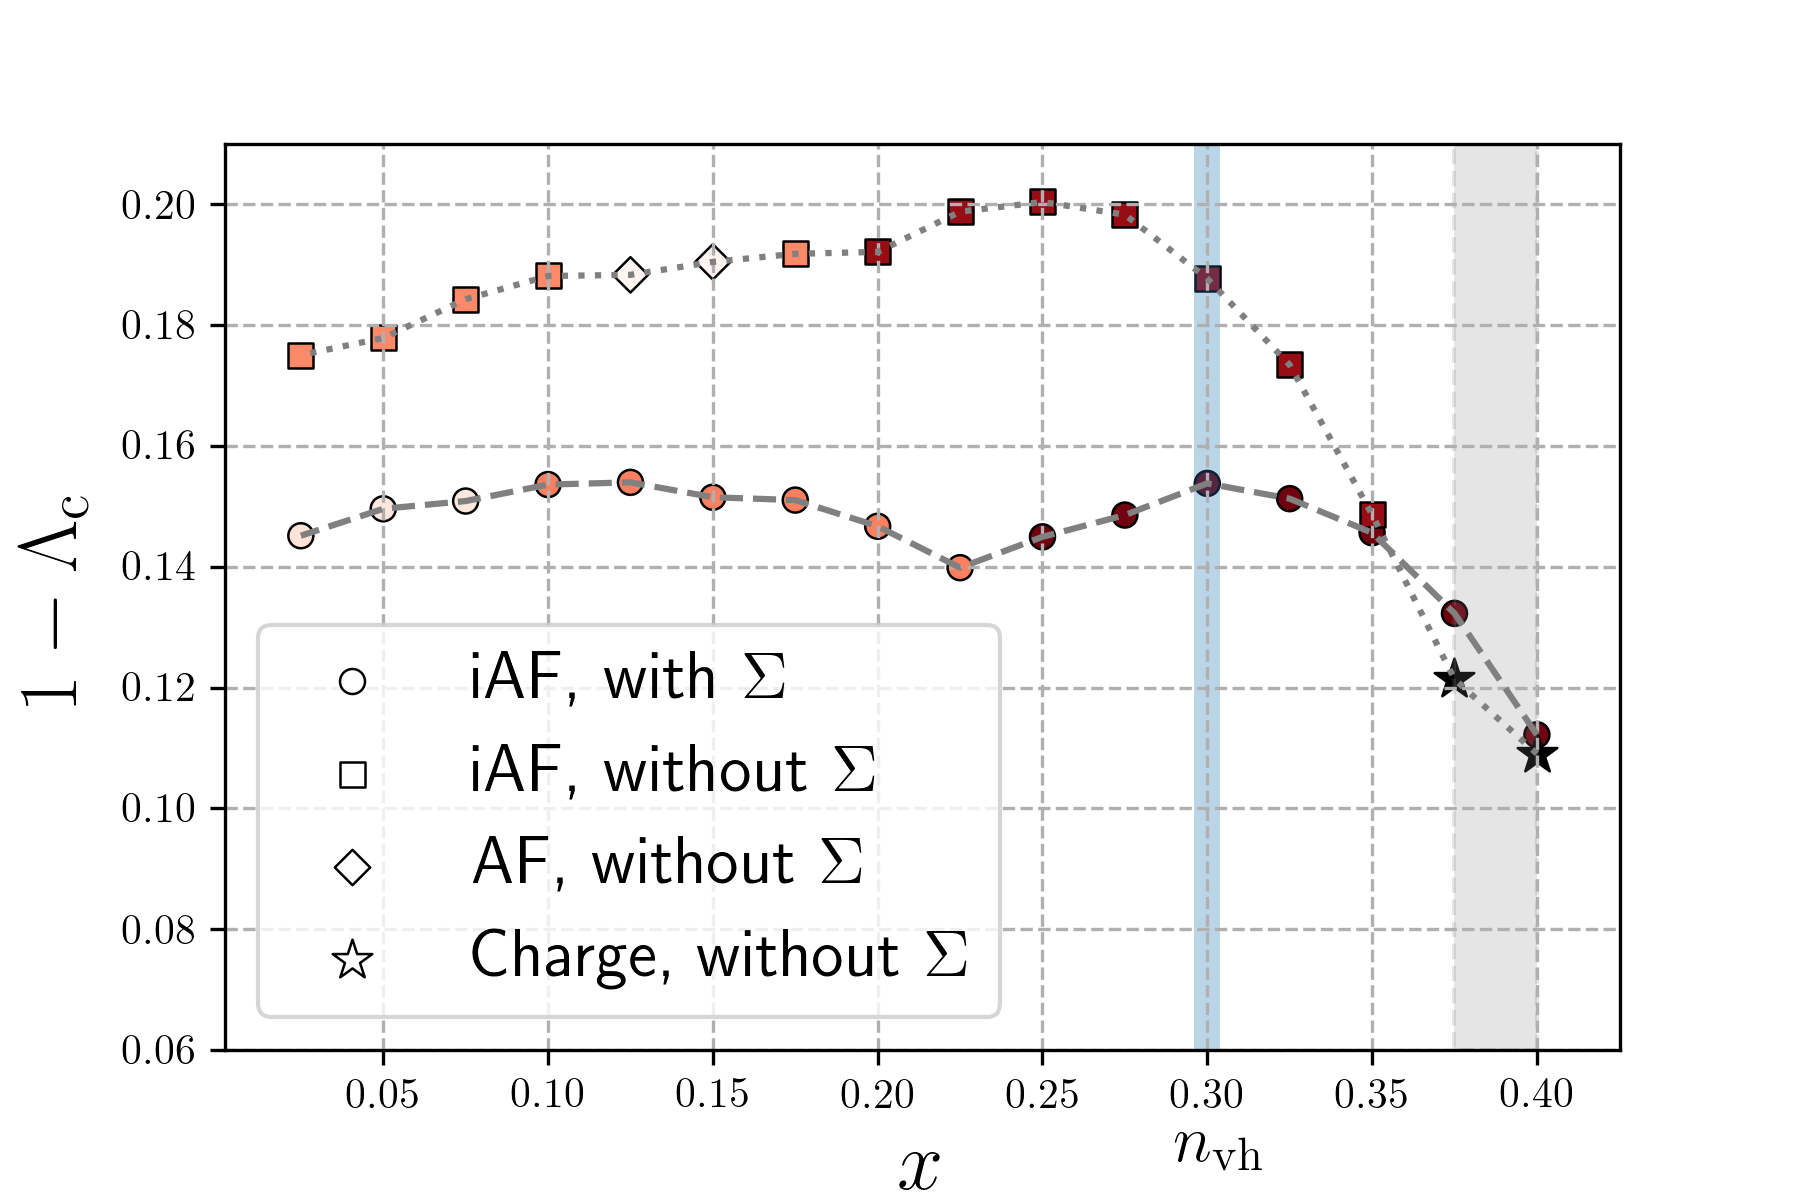
\includegraphics[width=0.5\textwidth]{images/phasediag.png}
\caption{Critical scale $1-\Lambda_{\mathrm{c}}$ as a function of the doping $x$, for $T = 0.08t$, $t'=-0.32t$ and $U=4t$. 
Square symbols and circles refer to incommensurate antiferromagnetism (iAF), respectively without and with self-energy feedback.
The black stars refer to a divergence in the charge channel (forward scattering). 
The color of squares and circles encodes distance of the incommensurability vector from $(\pi,\pi)$: darker color corresponds to higher incommensurability. }  
\label{fig:criscale} 
\end{figure}
In Fig. \ref{fig:criscale} we show the critical scale $1-\Lambda_{\mathrm{c}}$ as a function of the doping $x=1-n$ with and without self-energy feedback,  for $T=0.08t$, $t'=-0.32t$ and  $U=4t$.
In order to be consistent with previous fRG literature, we show our result as function of $1-\Lambda$, which vanishes at the end of the flow. 
For the physical interpretation, we can refer, instead, to the rescaled interaction $\tilde U ^\Lambda$.  


The critical value has been defined as the scale for which the value of  the larger channels exceeds $200t$. 
We have checked that for these stopping values the flow of the largest channel becomes to increase stronger than exponentially. These results are also consistent with an instability analysis based on the susceptibilities.        

The presence of the divergence signals a symmetry breaking at finite temperature, not compatible with the Mermin-Wagner theorem\cite{Mermin1966} since in our truncation-scheme we do not include the bosonic-fluctuations of the order parameter\cite{Baier2004}, essetial to obtain a vanishing critical temperature. 
The presence of a finite critical scale in the pure fermionic fRG signals the appearance of strong bosonic fluctuations that cannot be treated within the framework we are using. 
Even though the flow cannot be continued beyond the critical scale, from the analysis of vertex and self-energy at this scale we can identify the fluctuations that dominate the physics at low temperature.

In the specific case of the interaction cutoff we can interprete the rescaled interaction $\tilde U^{\Lambda_\mathrm{c}}$ as the critical interaction at a given temperature.

For the parameter set shown in Fig. \ref{fig:criscale} and without self-energy feedback, there are two possible instabies. 
For a doping smaller than $0.35$ the leading fluctations of the system are either commensurate antiferromagnetic or incommensurate antiferromagnetic. 
The incommensurability vector defined as $\mathbf{Q}=(\pi,\pi-\delta)$ corresponds to the momentum value for which the magnetic channel $\mathcal{M}^\Lambda$ has its maximum. The value of $\delta$ is encoded in the color of the symbols, where a darker color corresponds to a larger $\delta$, reaching the value of $\delta=1.13$ for a doping $x$ between $0.25$ and $0.35$. 
The region of commensurate antiferromagnetism for  $0.125\le x \le 0.150$ has to be attributed to the presence of a large plateu around $(\pi,\pi)$ in the bare bubble. Correspongingly the magnetic susceptibility is enhanced in all the region around $(\pi,\pi)$, and the commensurate peak cohexists with an incommensurate one, almost of the same magnitude.   
\begin{figure}
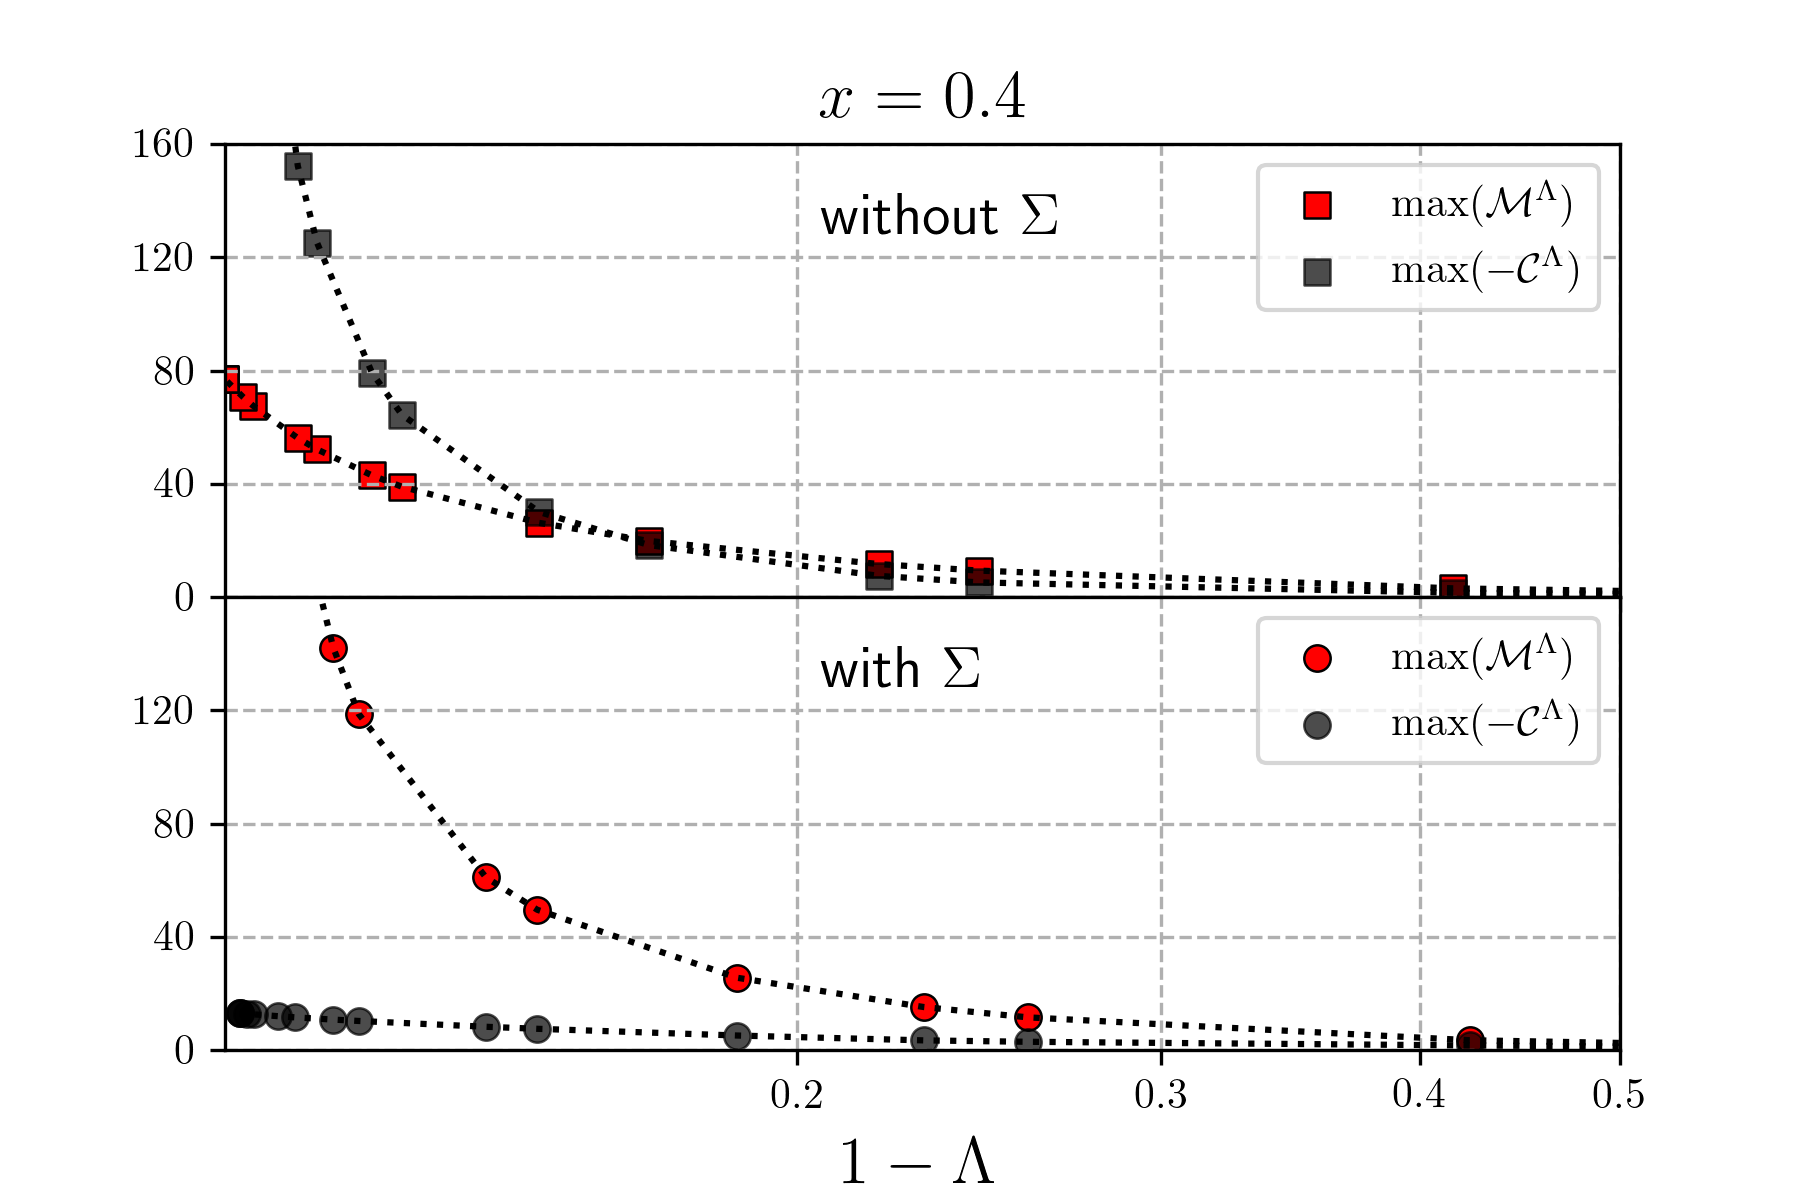
\includegraphics[width=0.45\textwidth]{images/chargeproblem_MC_vs_Lambda_fix_occ.png}
\caption{Flow of the maximal value of the charge channel $\mathcal{C}^\Lambda_{\Omega,\bs{Q}}(\nu_1,\nu_2)$ and of the magnetic channel $\mathcal{M}^\Lambda_{\Omega,\bs{Q}}(\nu_1,\nu_2)$ as a function of $\Lambda$, for  $x=0.4$, $t'=-0.32$, $U=4t$ and $T=0.08t$, without self-energy feedback (top) and with self-energy feedback (bottom). }
\label{fig:chargeproblem}
\end{figure}

The most striking feature is the presence of a divergence of the charge channel $\mathcal{C}^\Lambda$ for larger values of doping, marked in Fig. \ref{fig:criscale} by a black star. 
This feature was already observed by Husemmann \textit{et al.} in Ref. \onlinecite{Husemann2009}, where it was named \textit{forward scattering instability}. 
The charge channel $\mathcal{C}^\Lambda$ diverges for a finite frequency transfer $\Omega=2\pi/\beta$, which makes the interpetation of the divergence in terms of a physical instability not obvious. 
The frequency structure of the divergent charge channel $\mathcal{C}^\Lambda$, together with the one of the magnetic channel $\mathcal{M}^\Lambda$ is shown in Fig. \ref{fig:freqplot}, and will be discussed further in paragraph \textbf{addpara}.

\begin{figure}
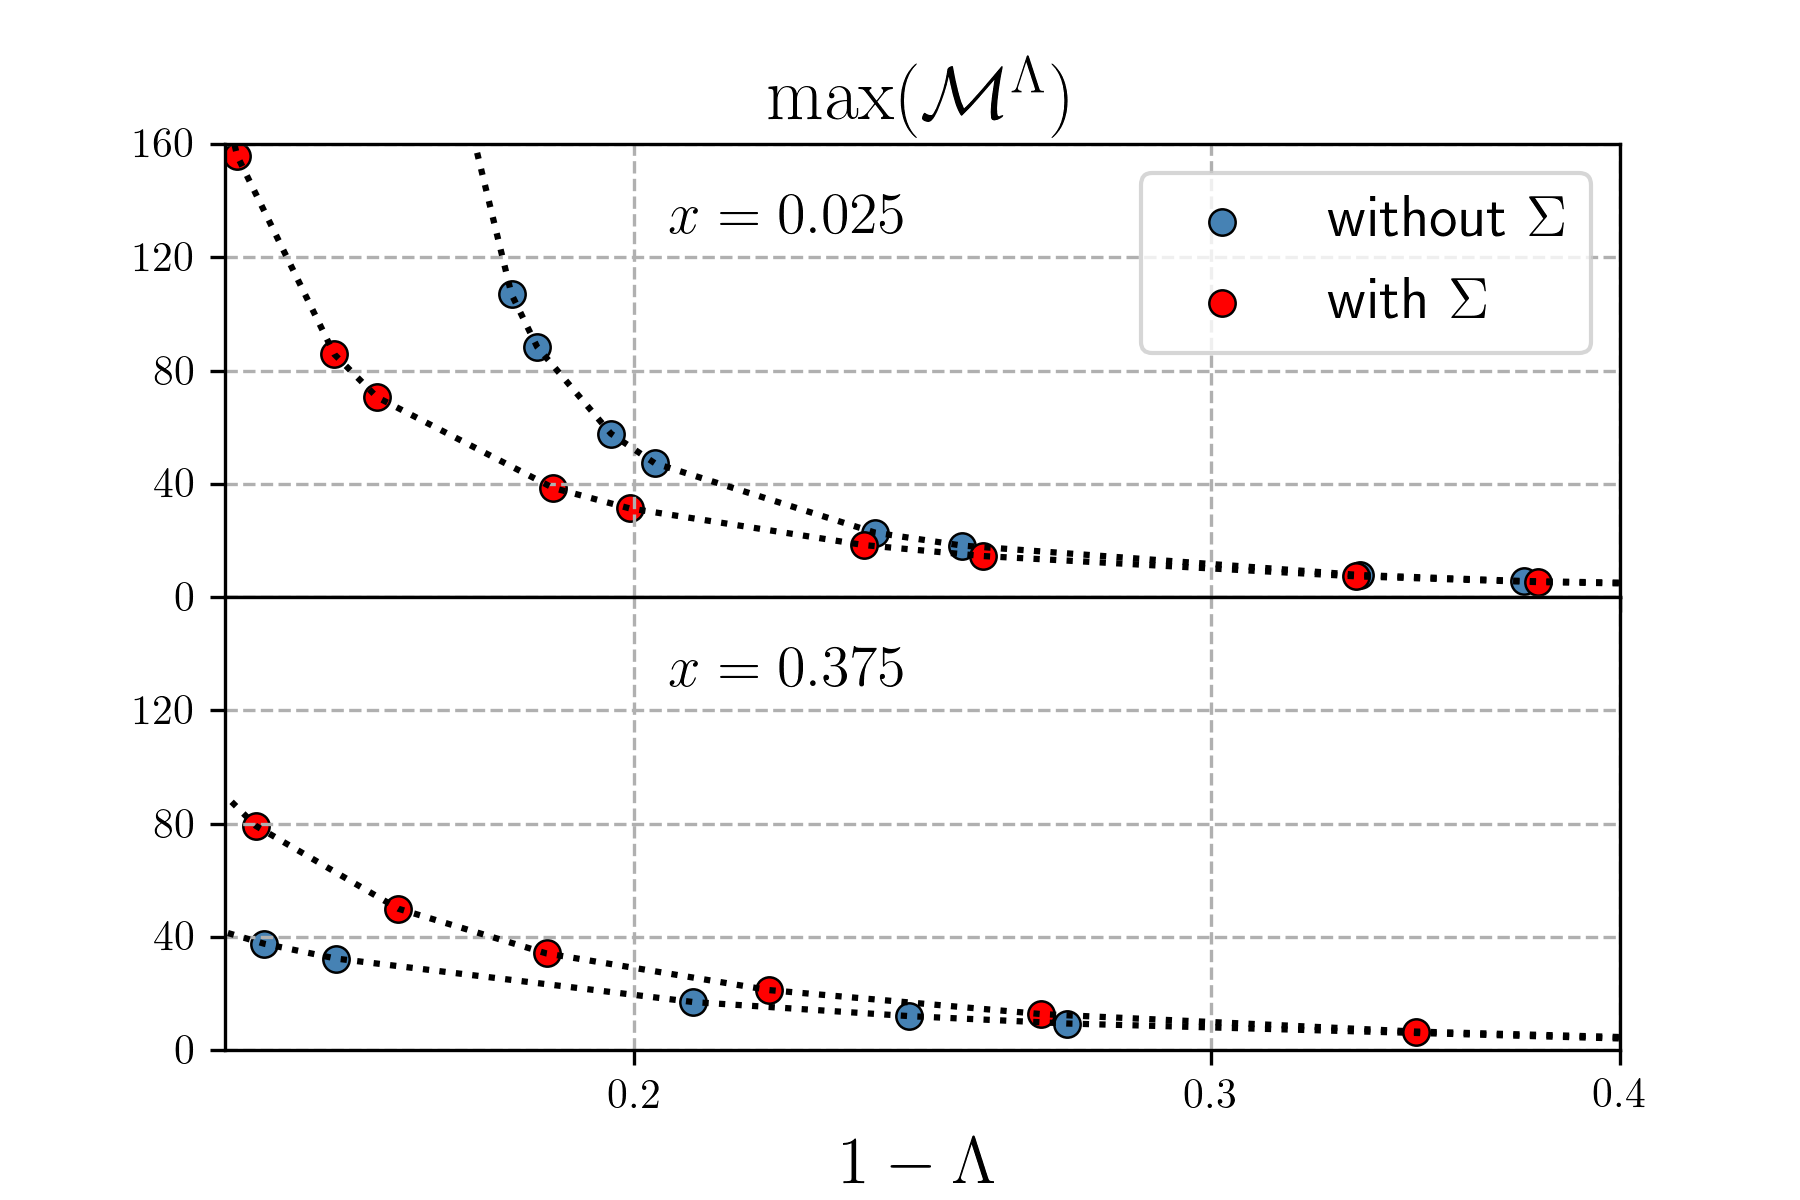
\includegraphics[width=0.45\textwidth]{images/chargeproblem_M_vs_Lambda_diff_occ.png}
\caption{Flow of the maximal value the magnetic channel $\mathcal{M}^\Lambda_{\Omega,\bs{Q}}(\nu_1,\nu_2)$ as a function of $\Lambda$, for $t'=-0.32$, $U=4t$ and $T=0.08t$ without self-energy feedback and with self-energy feedback. Top $x=0.025$, bottom $x=0.375$. }
\label{fig:selfeffect}
\end{figure}

Including the self-energy feedback results in three effects, as can be seen from Fig. \ref{fig:criscale}. 
First, $1-\Lambda_c$ is decreased.
Second, the incommensurability vector is also affected, the region of commensurate antiferromagnetism disappears, and one can observe a more regular trend of increasing $\delta$ as the doping is increased.
Finally, the divergence in the charge channel is completely suppressed, and the leading instability in the larger doping region studied  $0.4> x >0.375$ remains of the incommensurate antiferromagnetic type. 
This can be also be seen from Fig. \ref{fig:chargeproblem}, where we compare the flow of the maximum of the absolute value of magnetic and charge channel with and without the self-energy feedback. Without self-energy feedback, the charge channel rapidly starts to increase, taking large and negative values. Probably due to its feedback in the magnetic channel the latter never becomes particularly large.    
The effect of the self-energy feedback to the charge channel is dramatic: not only it does not diverge during the flow, but also it never exceeds a value of $15t$. 
On the other hand, due to the suppression of $\mathcal{C}^\Lambda$ the magnetic channel appears enhanced.
Hence the self-ennergy can affect the magnetic channel either directly, reducing the particle-hole bubble, or inderectly through the feedback of other channels.   
As we can see from the occupation-plot shown in Fig. \ref{fig:amoredidemetrio}, the effect of the self-energy on the Fermi surface is moderate, but enough to suppress the forward scattering instability. 

\begin{figure}
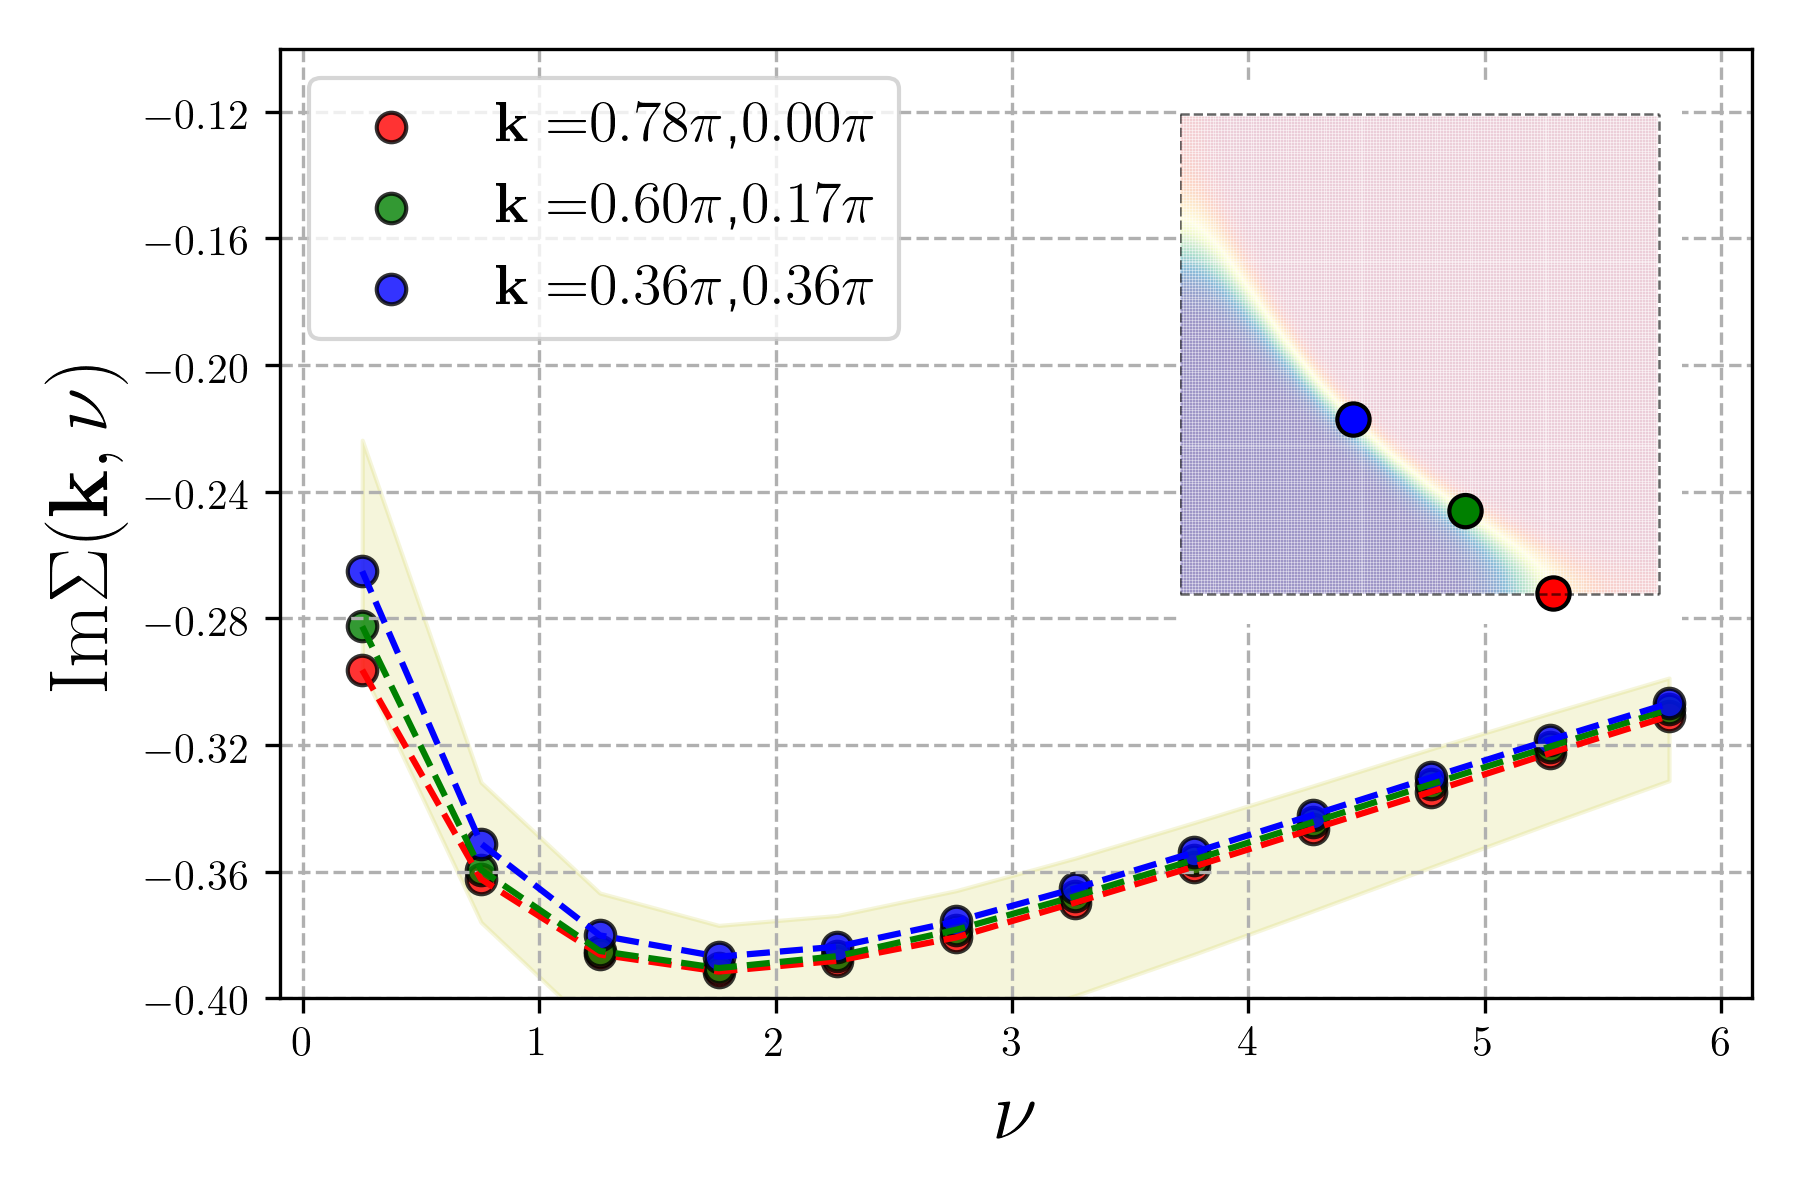
\includegraphics[width=0.45\textwidth]{images/Self_Im_occ0600.png}
\caption{Frequency dependent self-energy for parameter set... .
The location of the $\mathbf{k}$-point in the Brillouin zone is color coded in the inset. }
\label{fig:selffermi0600}
\end{figure}


\begin{figure}
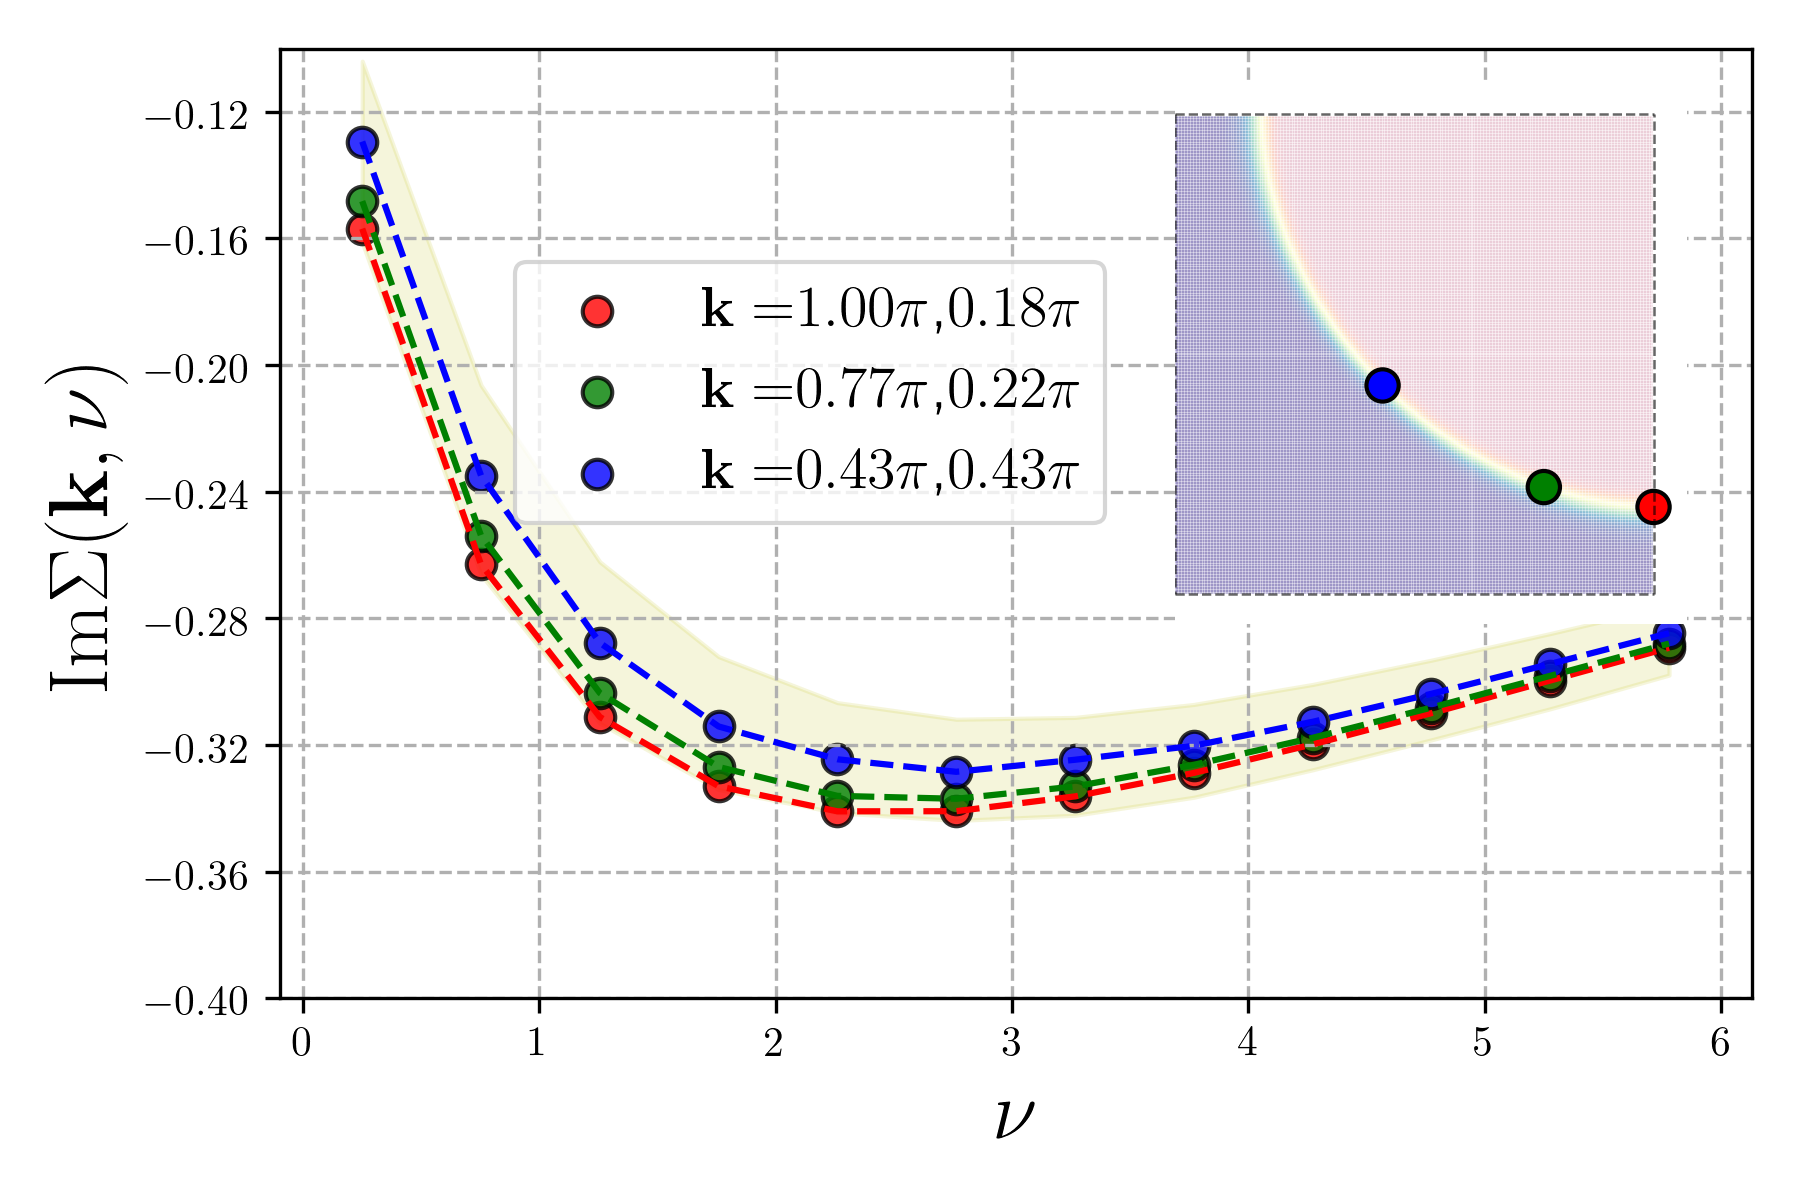
\includegraphics[width=0.45\textwidth]{images/Self_Im_occ0975.png}
\caption{Frequency dependent self-energy for parameter set... .
The location of the $\mathbf{k}$-point in the Brillouin zone is color coded in the inset. }
\label{fig:selffermi0975}
\end{figure}


All these considerations suggest that the divergence of the charge channel is rather an artefact of fRG without self-energy, arising from a lack of consistence between the vertex and the Green's function in the flow equations. 
In the next section we further substanciate this conclusion, by explaining the mathematical origin of the feature. 
The self-energy has qualitative and quantitive effects on the flow equations: quantitively 


\begin{figure}
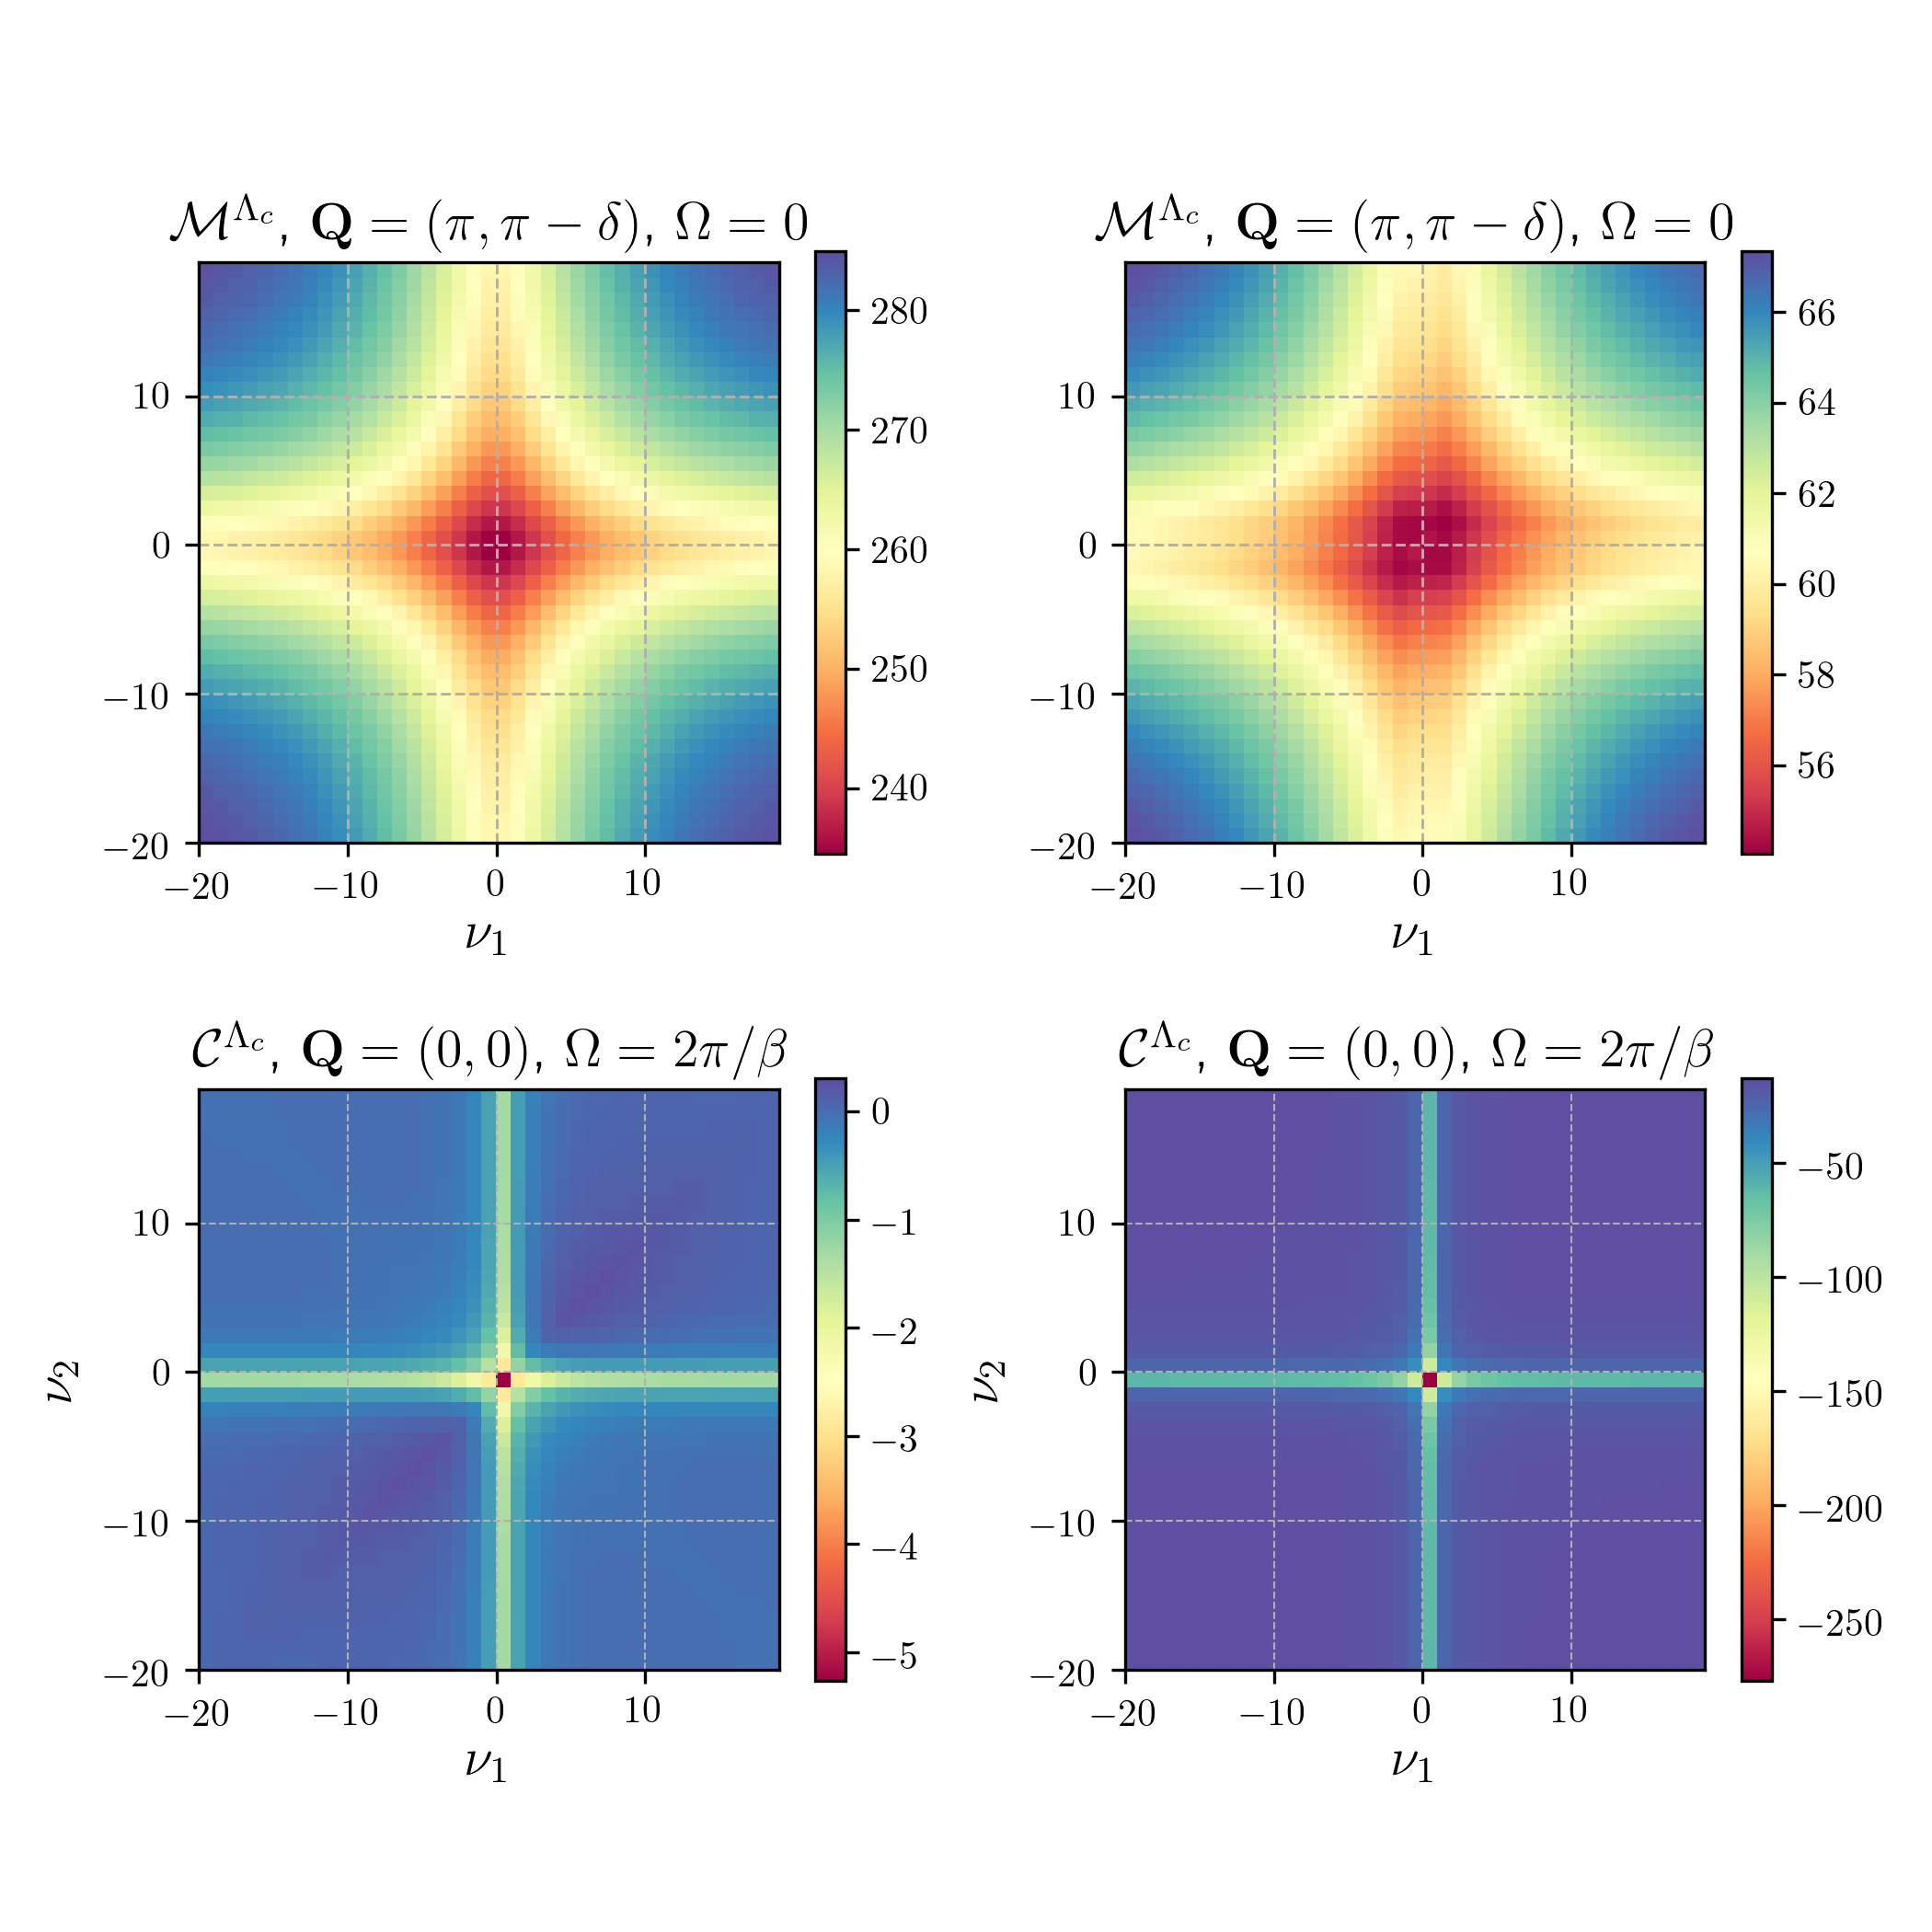
\includegraphics[width=0.45\textwidth]{images/Phi_color_all.png}
\caption{Frequency structure of the charge channel $\mathcal{C}^\Lambda_{\Omega,\bs{Q}}(\nu_1,\nu_2)$ (on the left) and of the magnetic channel $\mathcal{M}^\Lambda_{\Omega,\bs{Q}}(\nu_1,\nu_2)$ (on the right), for $x=0.4$, $t'=-0.32$, $U=4t$ and $T=0.08t$ and without self-energy, corresponding to the rightmost point in Fig. \ref{fig:criscale}. 
Both channels are plotted for the frequency and momentum transfer for which they have their maximum. Note that the frequency transfer for $\mathcal{C}^\Lambda_{\Omega,\bs{Q}}$ is the first bosonic Matsubara frquency $2\pi/\beta$. 
The value of $\delta$ is $1.13$.  
 }  
\label{fig:freqplot} 
\end{figure}


\begin{figure}
%\hspace*{-1.5cm}
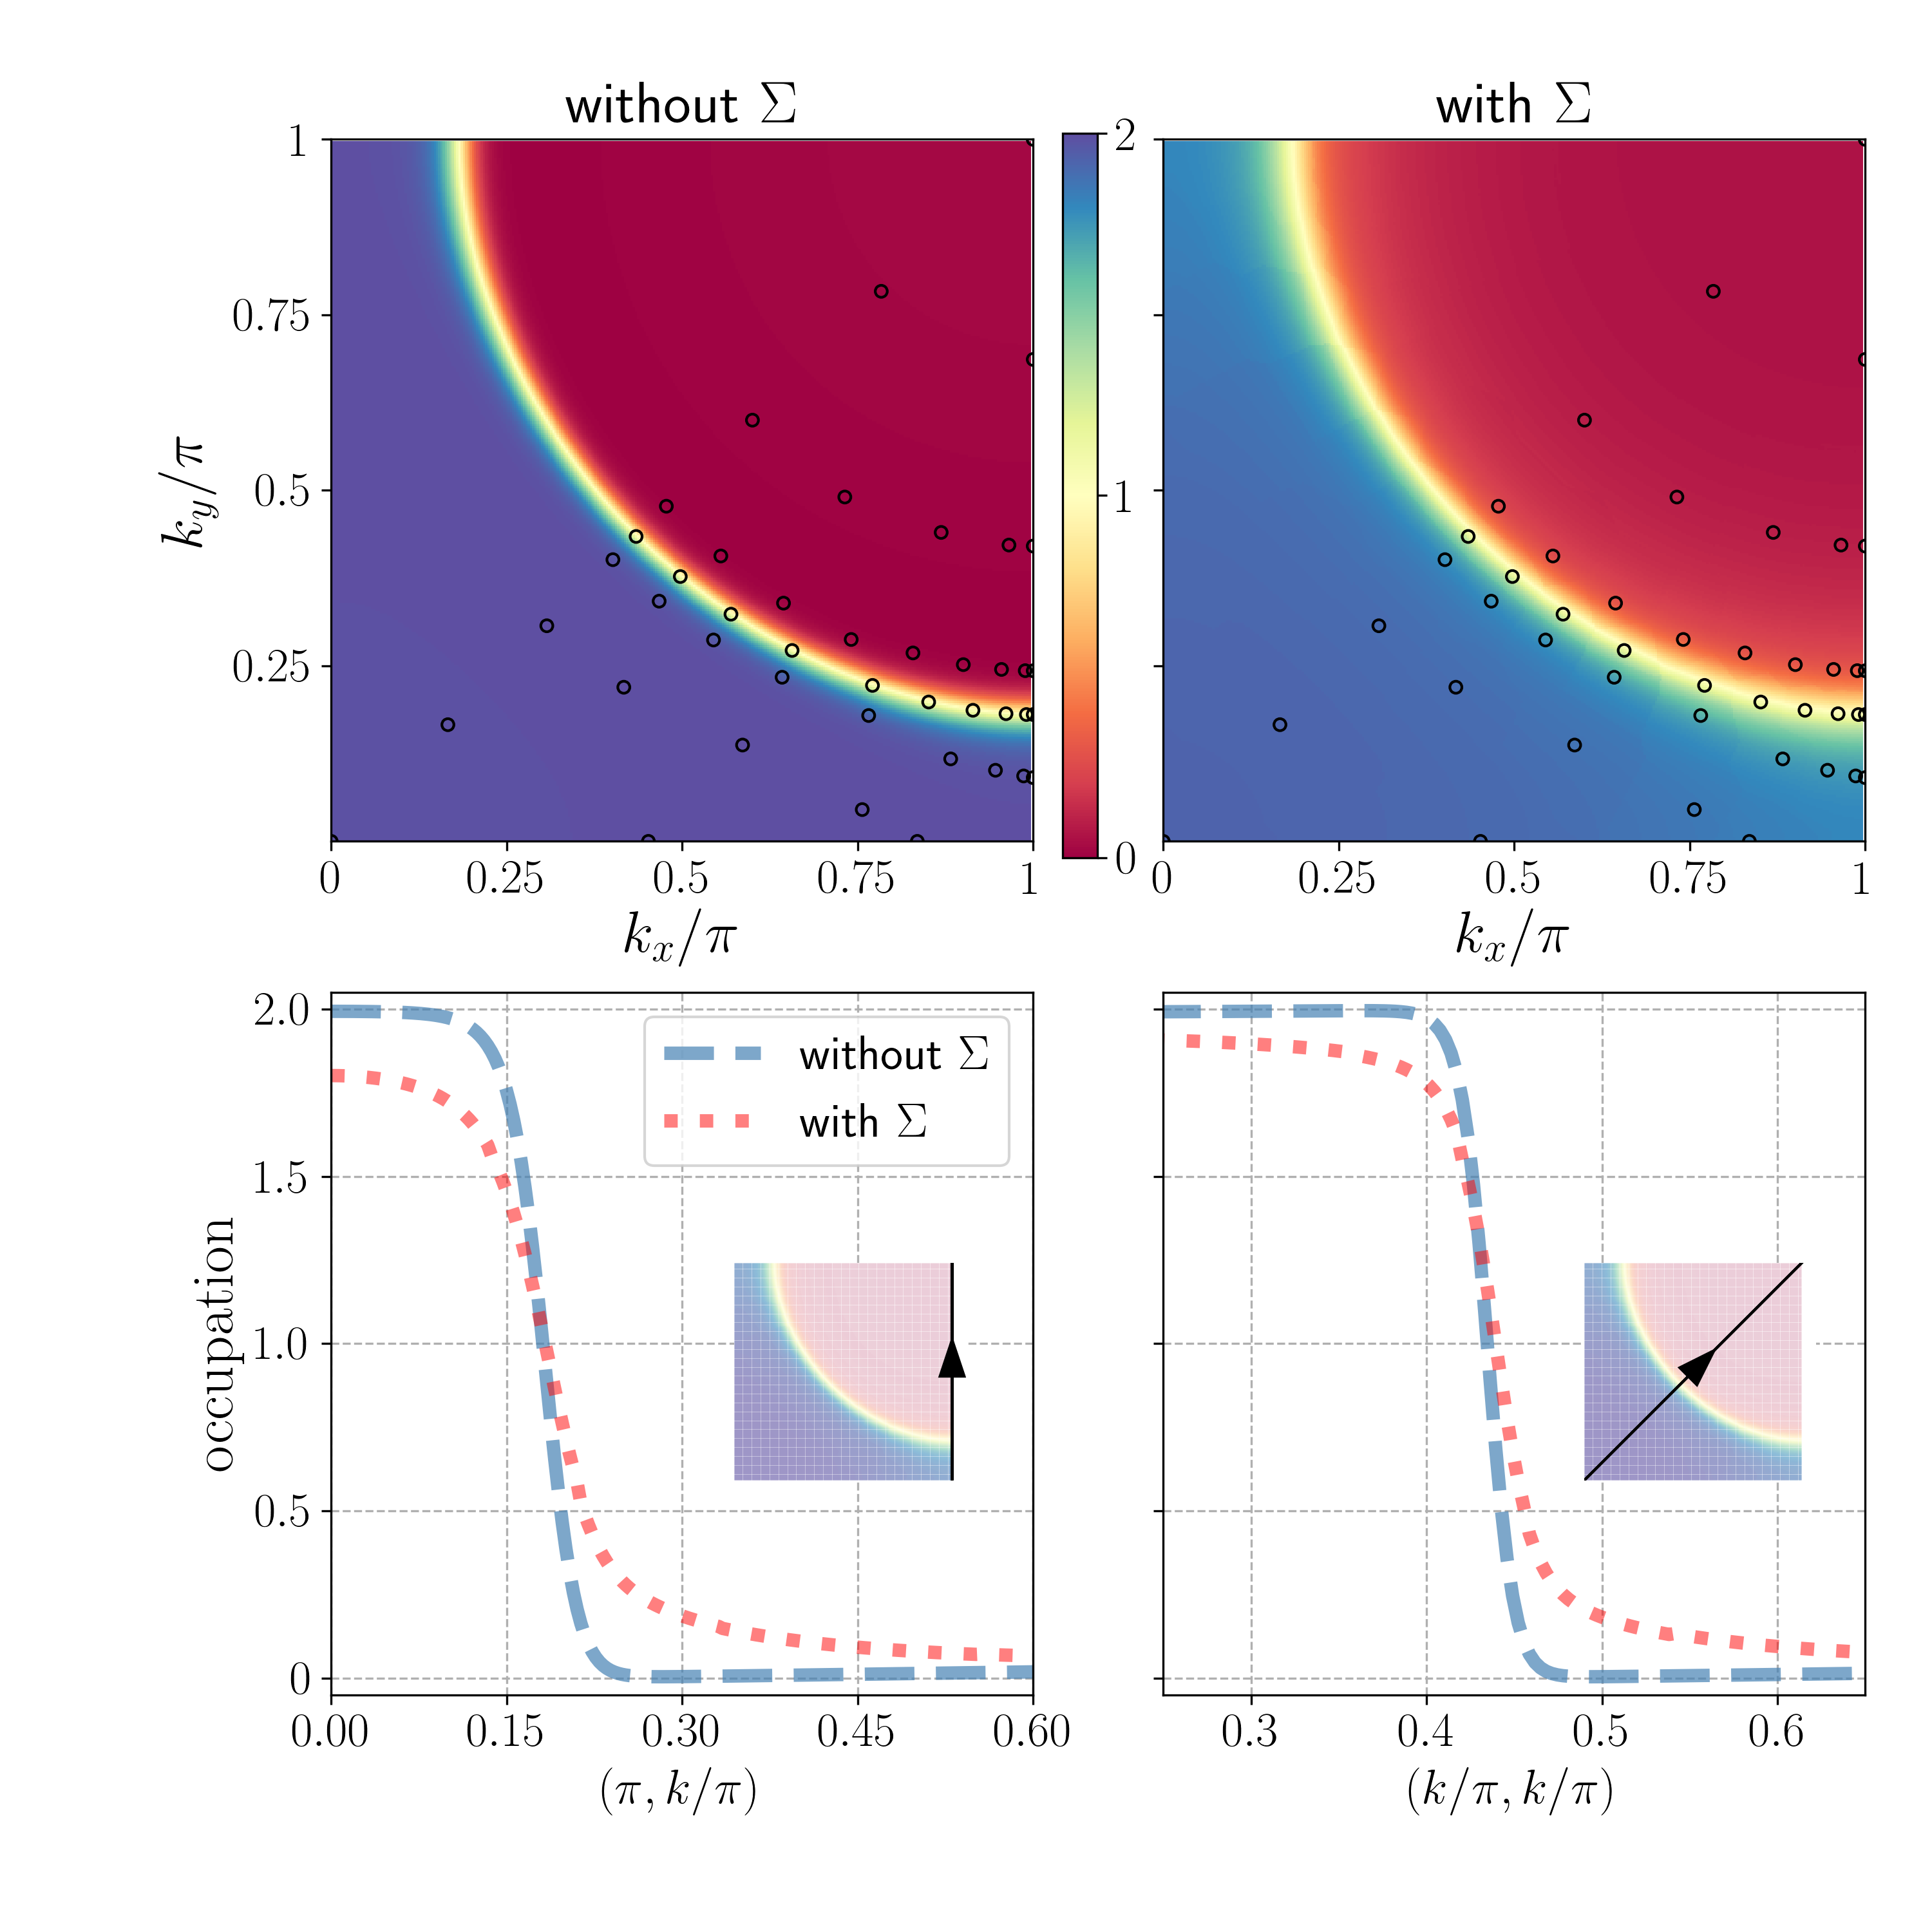
\includegraphics[width=0.5\textwidth]{images/occupations_0975.png}
\caption{\textbf{placeholder}} 
\label{fig:occupation}
\end{figure}

\begin{figure}
%\hspace*{-1.5cm}
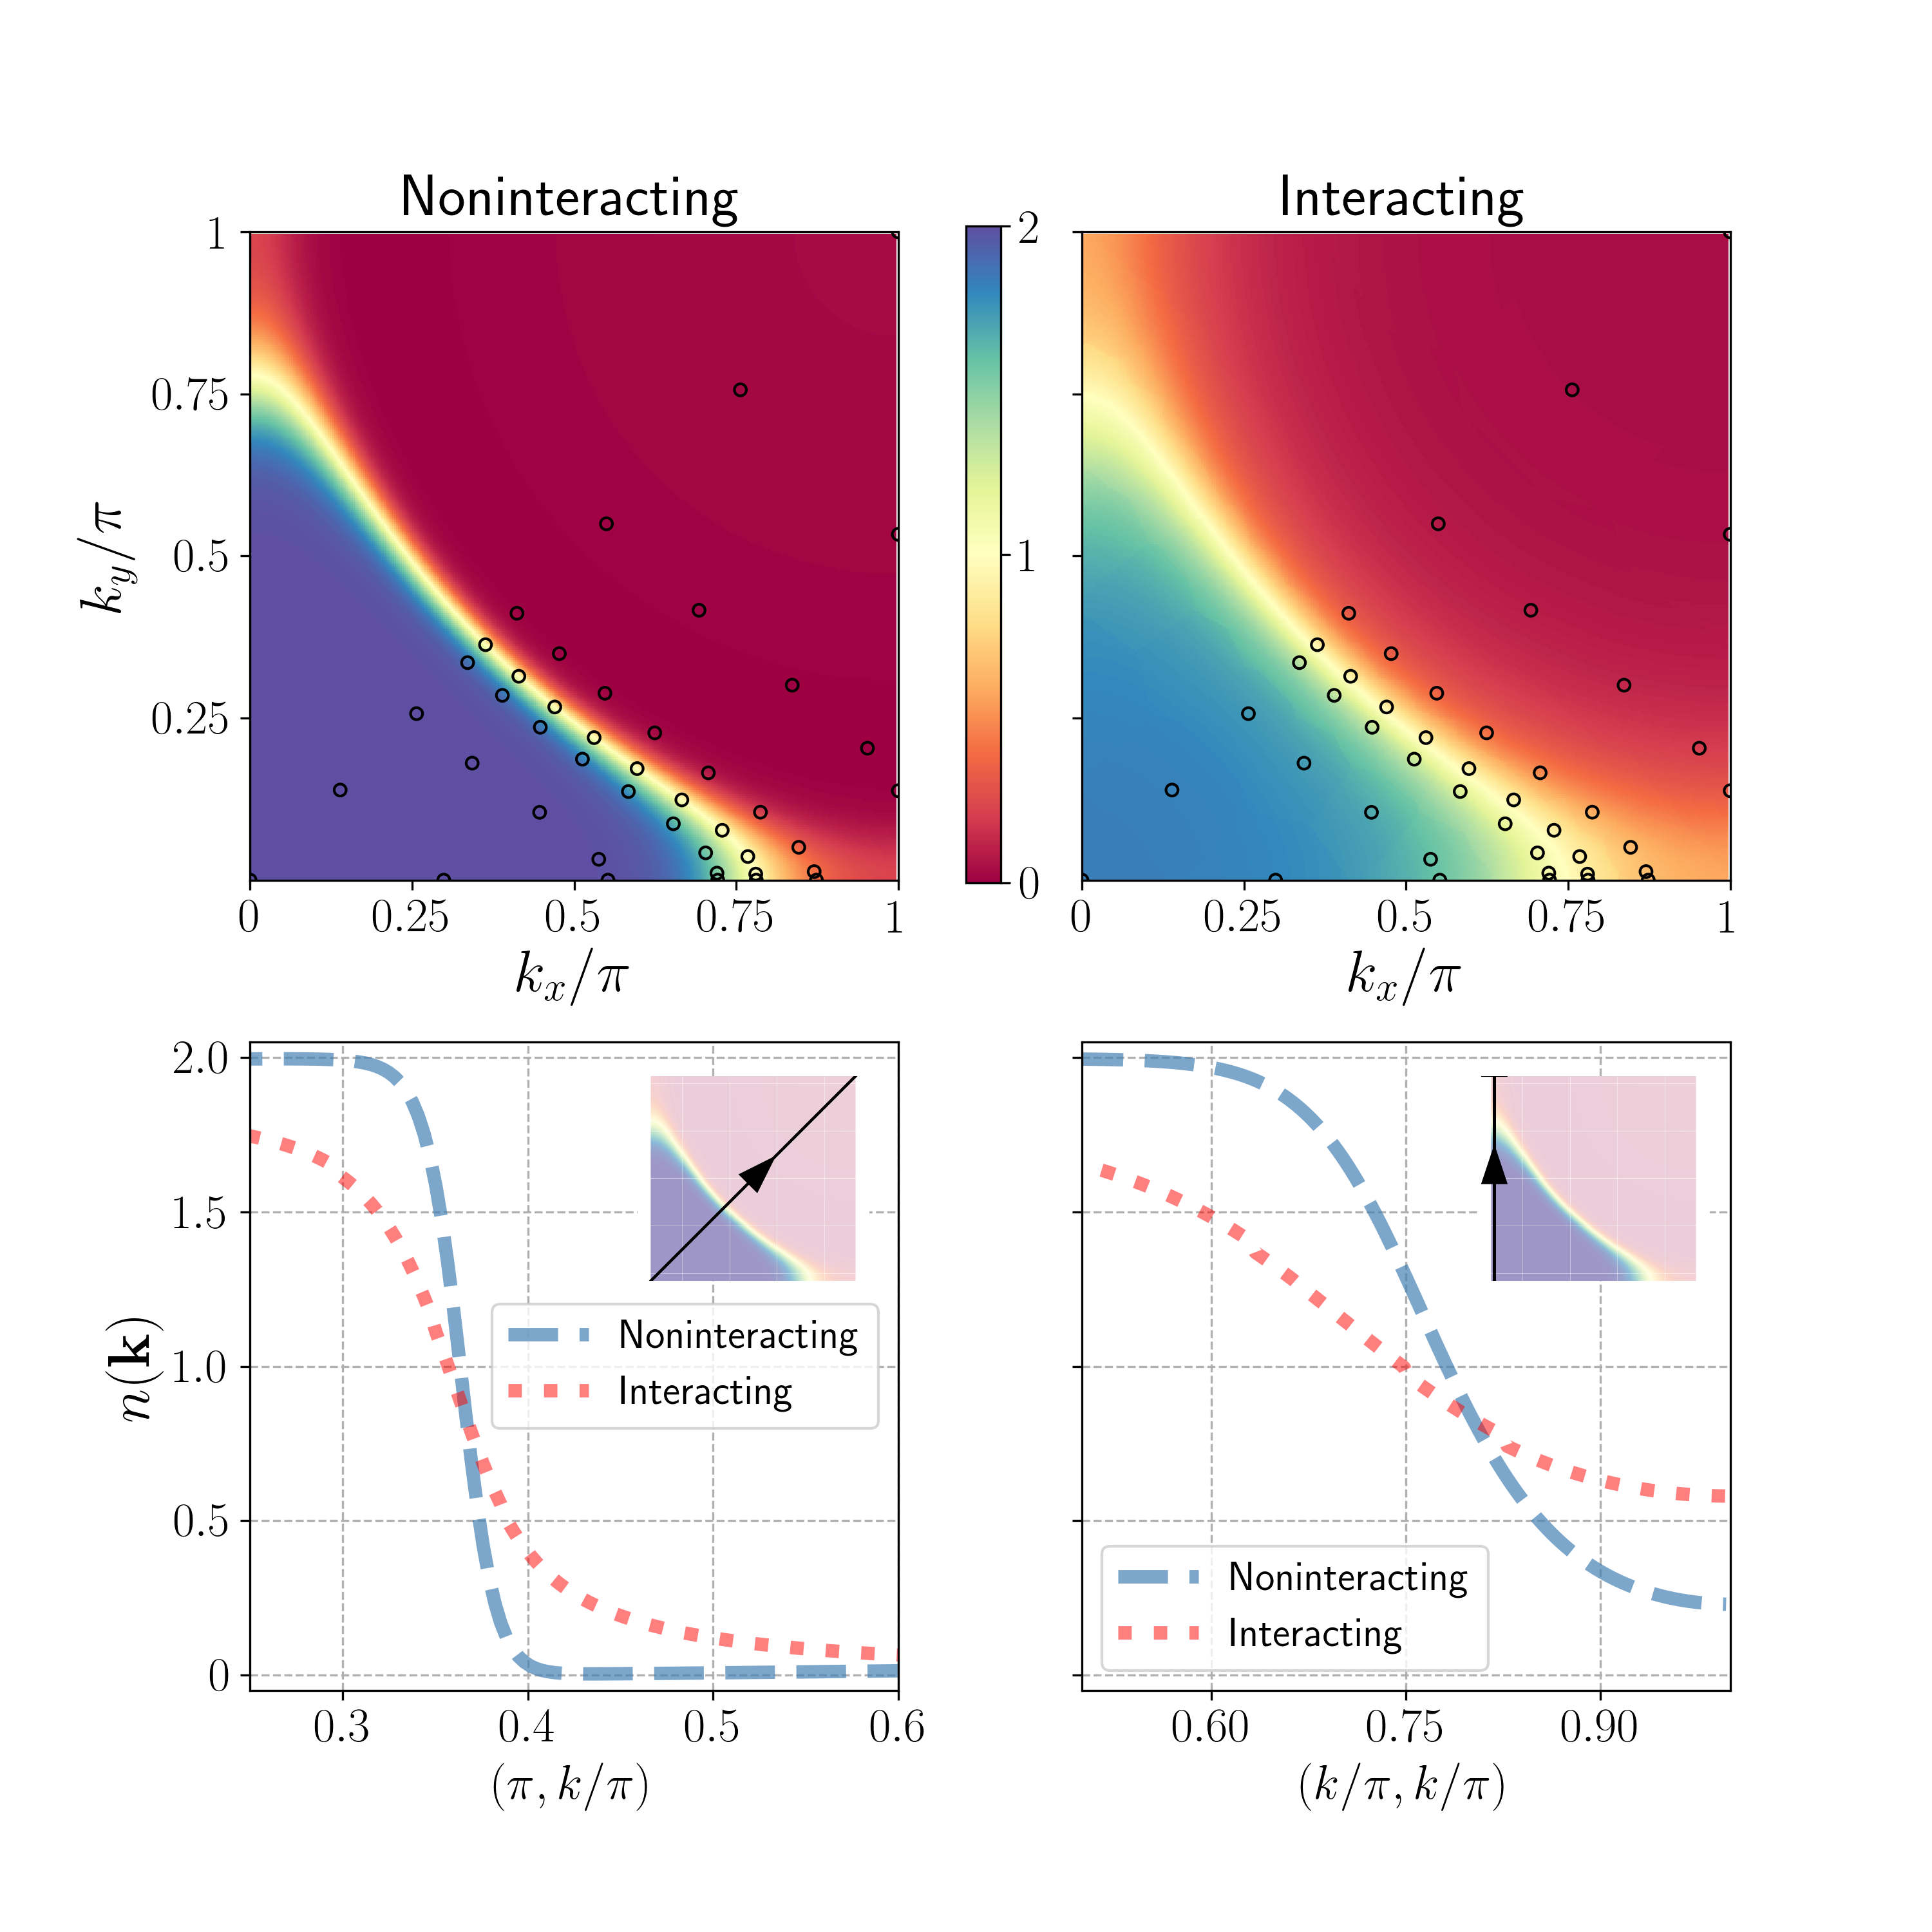
\includegraphics[width=0.5\textwidth]{images/occupations_0600.png}
\caption{\textbf{placeholder}} 
\label{fig:occupation}
\end{figure}





\begin{itemize}
\item interpretazione scala divergenza
\item notare charge problem con riferimento MS 
\item self energy vs no self energy
\item interaction  
\end{itemize}   


\subsection{Forward scattering problem}

\begin{figure*}
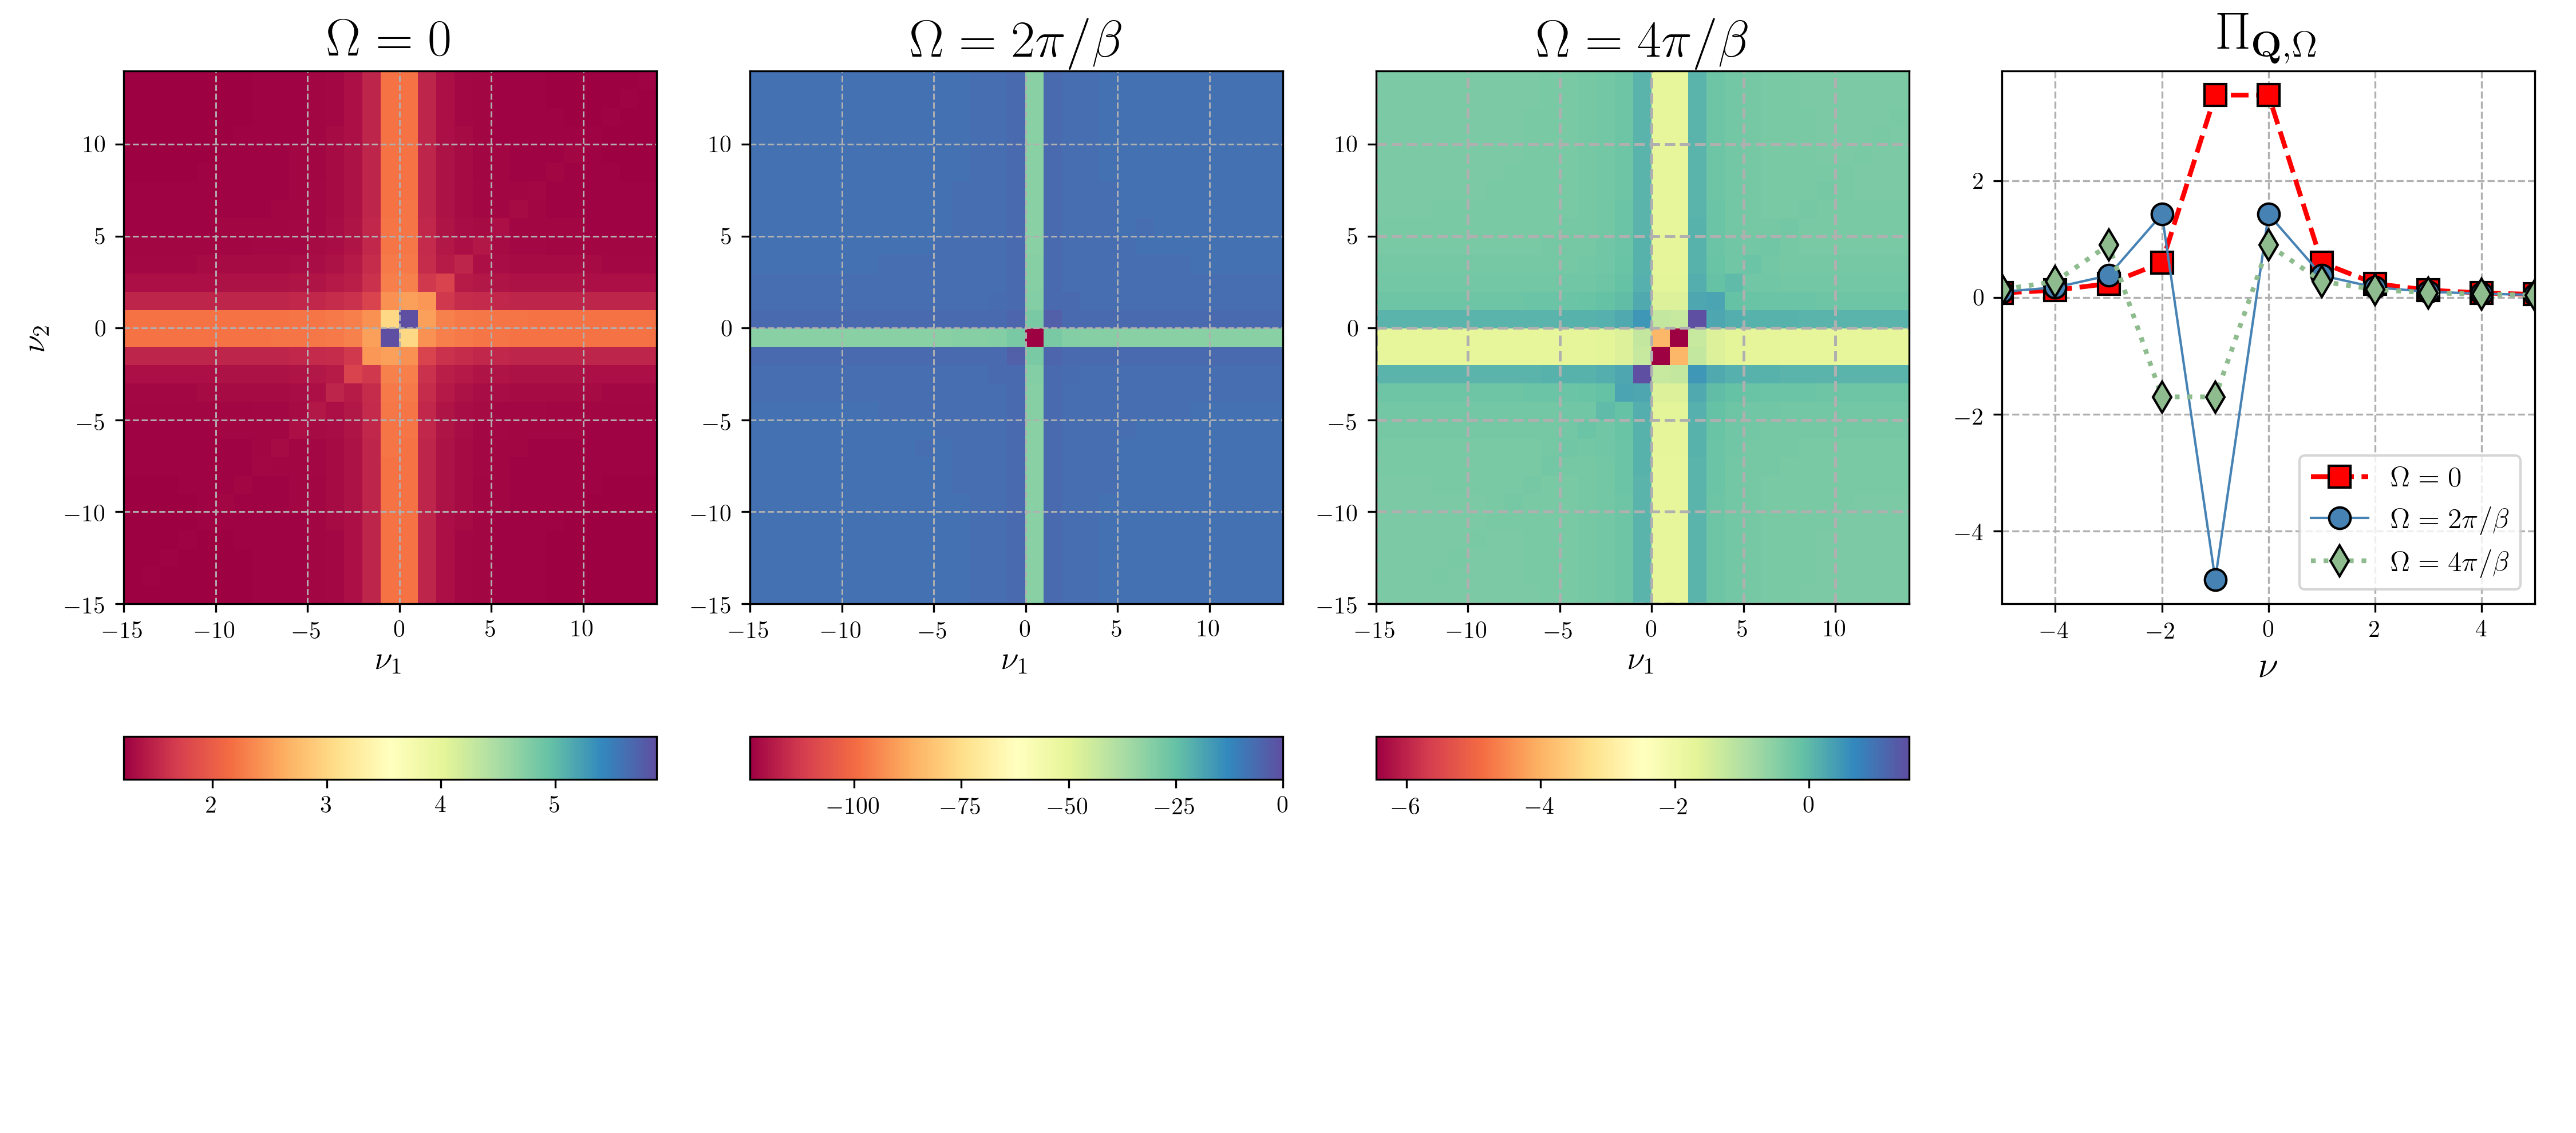
\includegraphics[width=\textwidth]{images/PL_all.png}
\caption{\textbf{placeholder}} 
\label{fig:perpladder}
\end{figure*}


\begin{itemize}

\item Introduce perpendicular ladder (PL) for charge.

\item Colorplot of charge in PL.

\item Discuss the role of the Bubble at $\boldsymbol{Q}=(0,0)$ and plot it as a function of $\nu$.

\end{itemize}

\subsection{Self energy analysis}

\begin{figure}
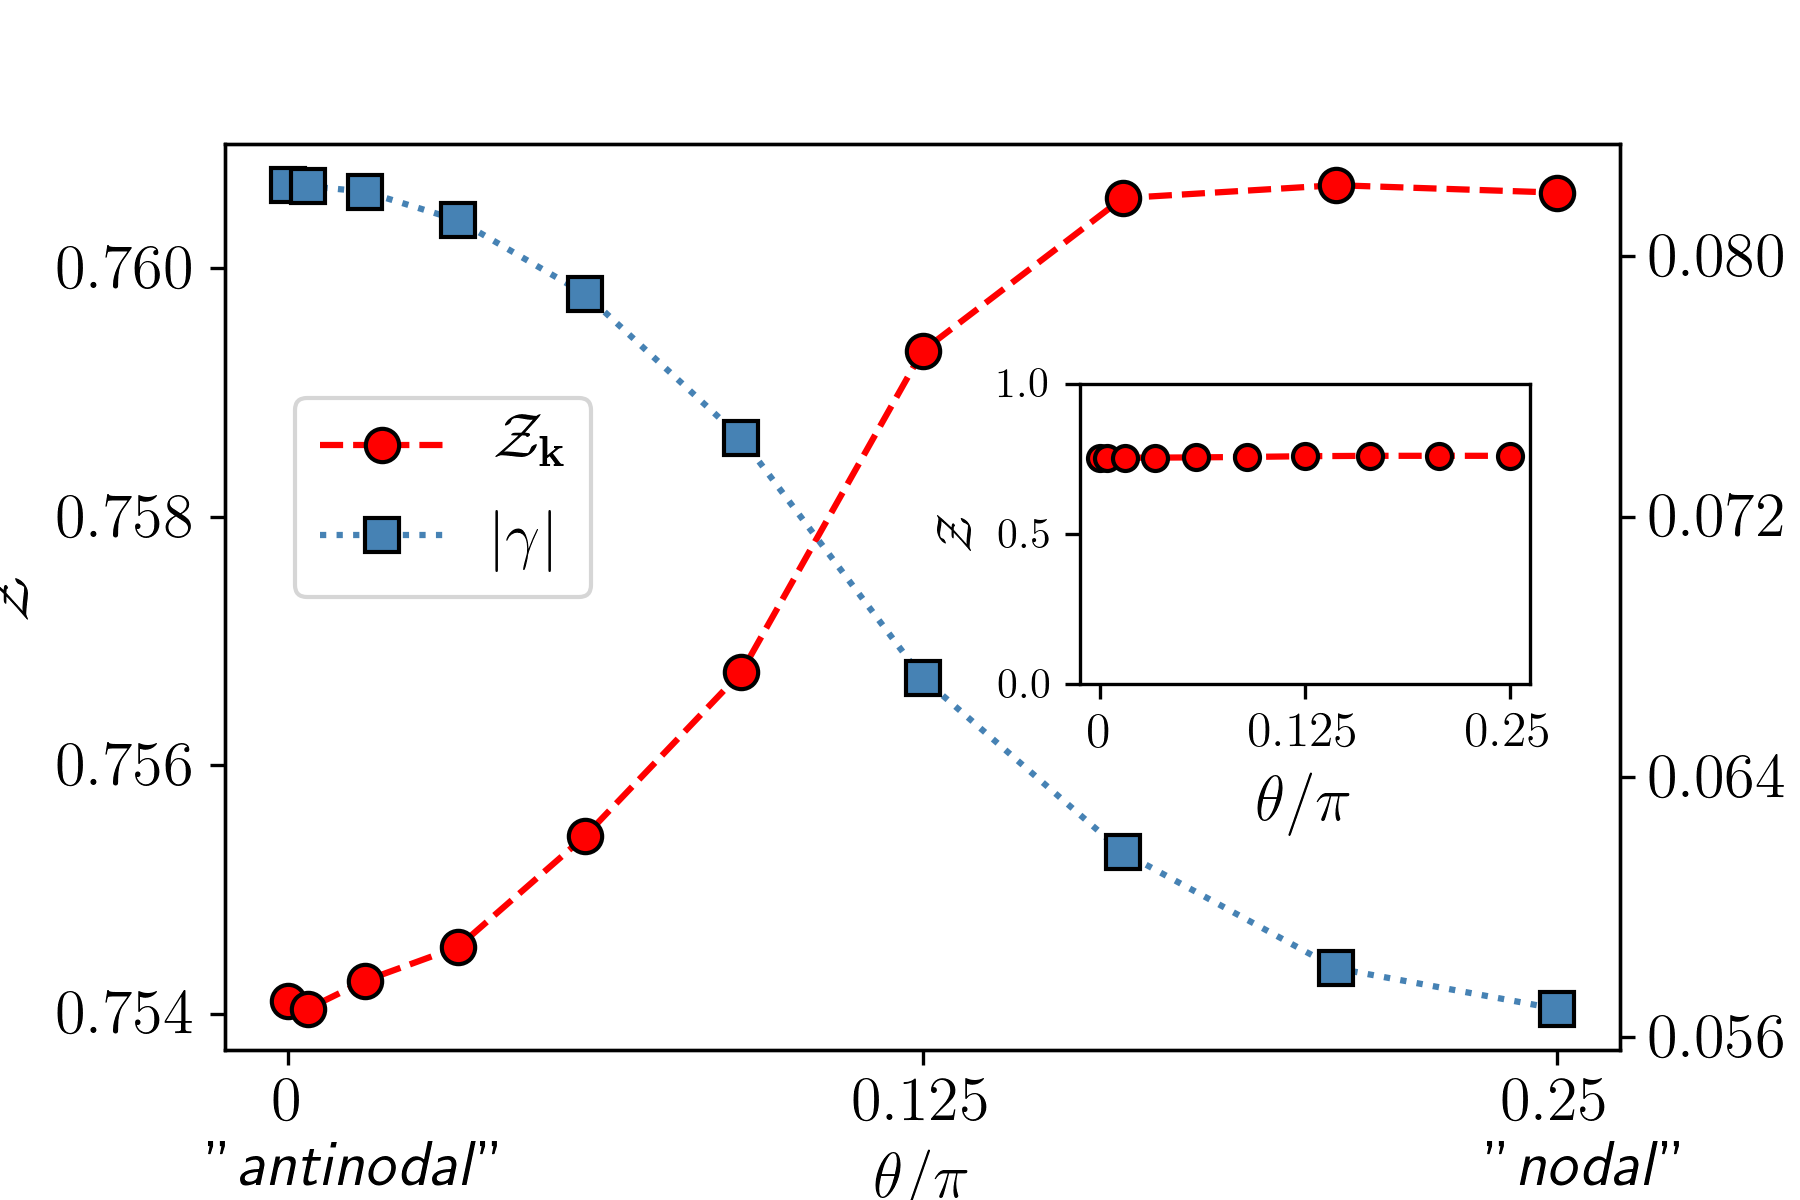
\includegraphics[width=0.4\textwidth]{images/z_and_gamma975.png}
\caption{\textbf{placeholder} }
\label{fig:zetaandgamma}
\end{figure}

\begin{itemize}

\item With self energy feedback, we didn't find any charge instability problem for any parameters range studied.

\item Plot of the Fermi surface based patch scheme.

\item Plot of $\Sigma(i\omega)$ at $\boldsymbol{k}=(\pi,0)$, $\boldsymbol{k}=\boldsymbol{k}_{HS}$ and $\boldsymbol{k}=(\pi/2,\pi/2)$ in frequency space.

\item Plot of $Z_{\boldsymbol{k}}$

\item Plot of occupation with and without $\Sigma$

\end{itemize}
